%%%%%%%%%%%%%%%%%%%%%%%%%%%%%%%%%%%
% PART II: Experiment definition module
%%%%%%%%%%%%%%%%%%%%%%%%%%%%%%%%%%%

\index{norm}{AEDL@\AEDL|(}
\part{The Abstract Experiment Definition Language -- AEDL}
\label{part:2}

\chapter{Getting started}

Here the general concept of the AEDL is described and illustrated by an example. In addition, a short introduction to the syntax of the AEDL is given.

\section{General concept of the experiment simulation}

The goal of AEDL is to describe a large number of complex and very 
different experiments by a limited number of parameters. It allows a
representation of very different setups within one data structure, and thus implements universal rate and $\chi^2$ computation methods. For experiment simulations, usually a new piece of code is written and compiled
for each different experiment. In many cases, even parameter changes, such as
the number of bins, require the recompilation of the source code. 
However, such a technique soon reaches its limits when the simulated experiments are rather complex, or more than one type of experiment is studied simultaneously. Furthermore, it is very difficult to verify the correctness of the obtained results, since every time a new piece of code is added to 
deal with a new experiment type, new errors will be introduced.

Thus, a general and flexible experiment description language is needed.  
The description of a neutrino experiment can be split into three parts: Source, oscillation, and detection. The neutrino sources within \GLOBES\ 
are assumed to be stationary point sources, where each experiment has only 
one source. This restricts the classes of neutrino sources which can be studied with \GLOBES :
\begin{itemize}
\item
 Experiments using many point-like sources can only be approximated. One example are reactor experiments using many distant reactor blocks.
\item
 Geometrical effects of a source distribution, such as in the sun or the atmosphere, can not be described.
\item
 Sources with a physically significant time dependency  can not be studied, such as  supernov\ae. It is, however, possible
to study beams with bunch structure, since the time dependence of the
neutrino source is physically only important to suppress backgrounds. 
\end{itemize}

The description of the neutrino oscillation physics is, at least numerically, relatively simple. We use the {\em evolution operator method}~\cite{Ohlsson:1999um}  to compute the neutrino oscillation probabilities and divide the matter density profile into layers of constant matter density. For each of these layers, the Hamiltonian in matter is diagonalized in order to propagate the neutrino transition amplitudes. Finally, the transition probability is obtained by the absolute square of the total neutrino transition amplitudes. Depending on the precision of the studied experiment, this approach turns out to be precise enough in Earth matter even if only a small number matter density steps is used. Since we allow an uncertainty of the matter density profile, it is, in fact, in most cases sufficient to consider only one density step with the average matter density together with a matter density uncertainty~\cite{Ohlsson:2003ip}. Note that this approach may not be applicable to quickly varying extraterrestrial matter density profiles.

While it is comparatively simple to define a general neutrino source 
and to compute the oscillation physics, the general properties of a detector simulation are much more complicated. The basic assumption in building an abstract detector description is \emph{linearity}, \ie , that two neutrino events do not interfere with each other. Furthermore it is assumed that all information on the oscillation physics 
is given by the \emph{reconstructed} flavor and energy of a 
neutrino event. The term ``reconstructed'' implies that the well-defined energy of the incident neutrino, which can not be directly observed, translates via secondary particles and the detection properties into a distribution of possible energy values. This process is illustrated in \figu{distro} for the energy variable. 
%
\begin{figure}[ht]
\begin{center}
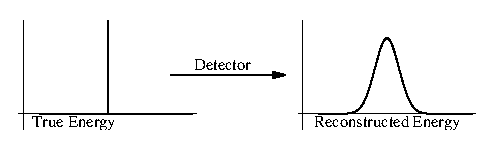
\includegraphics[width=0.6\textwidth]{mapping}
\end{center}
\caption{\label{fig:distro} A detector maps a true parameter value onto
a distribution of reconstructed parameter values. This is illustrated here for there energy.}
\end{figure}
% 
The same, in principle, applies to the nature of the neutrino flavor. However, in this case only discrete values are applicable. Note that the reconstructed neutrino energy and the neutrino flavor are the only observables in \GLOBES .

This picture can also be formulated in a more mathematical way. Let us define $x$ as the true parameter value and $x'$ as the reconstructed parameter value. Similarly, $f(x)$ is the distribution of true parameters values and $p(x')$ is the distribution of reconstructed parameter values. Then the detector function  $D(x,x')$, which describes the mapping performed by the detector, is given by
\begin{eqnarray}
\label{equ:mapping}
p(x')&=&\int dx\, f(x)\cdot D(x,x')\,.
\end{eqnarray}
Obviously \equ{mapping} only describes the detector properly
if the linearity condition is fulfilled. Within this model, a detector
is completely specified by a set of $D(E,E')$ for the energy variable $E$,
and a set $D(F,F')$ for the flavor variable $F$. In general, $D(E,E',F)$ also depends on the incident neutrino flavor $F$, as well as $D(F,F',E)$ depends on the incident neutrino energy $E$. These sets of mapping functions usually are obtained from a 
full detector simulation and can be obtained by using as input 
distribution $f(x)$ a delta distribution $\delta(x-x_0)$.

\begin{figure}[t]
\begin{center}
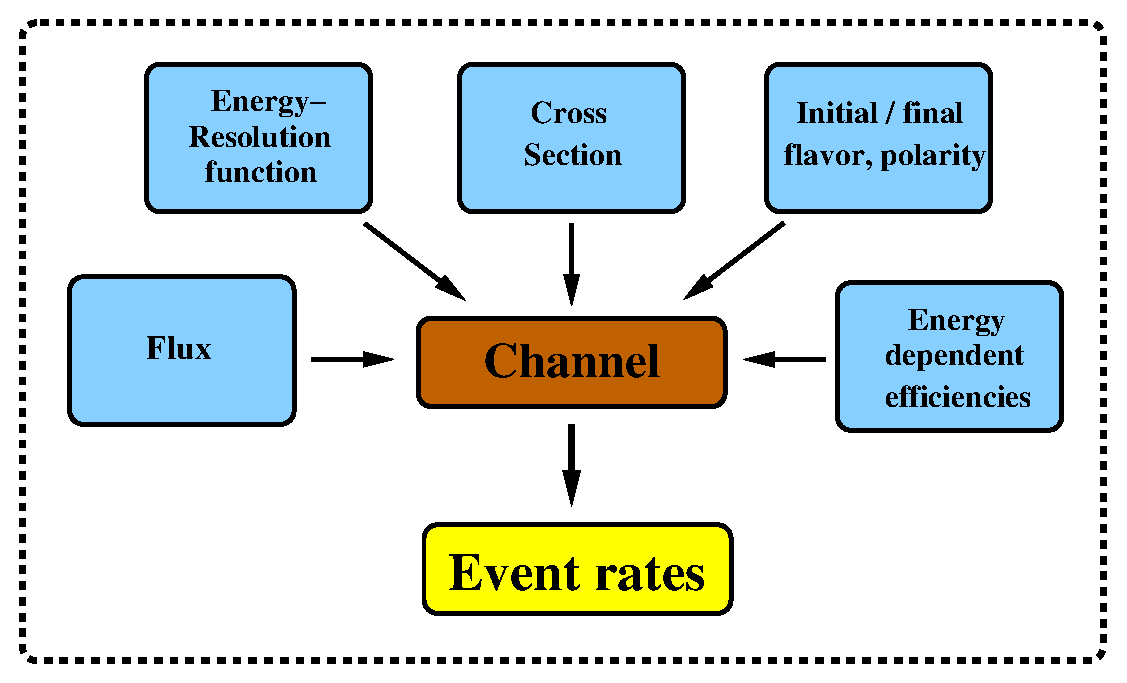
\includegraphics[width=13cm]{AEDL1}
\end{center}
\caption{\label{fig:channel} General concept of a ``channel''.}
\end{figure}

In order to implement a experiment definition including various
sources of systematical errors, we use several abstraction levels. 
The first level is the so-called ``channel'', \index{norm}{Channel}
 which is the link between 
the oscillation physics and the detection properties for a specfific oscillation pattern (\cf, \figu{channel}). A channel specifies the mapping of a specific neutrino flavor produced by the source onto a reconstructed neutrino flavor.
For example, a muon neutrino oscillates into an electron neutrino and subsequently interacts via quasi-elastic charged current scattering. The measured energy and direction of
the secondary electron in the detector then allows to reconstruct the neutrino energy. The connection from the source flux of the muon neutrino, via the  probability to appear as a electron neutrino, to its detection properties (such as cross sections and energy smearing) is encapsulated into the channel.

\begin{figure}[t]
\begin{center}
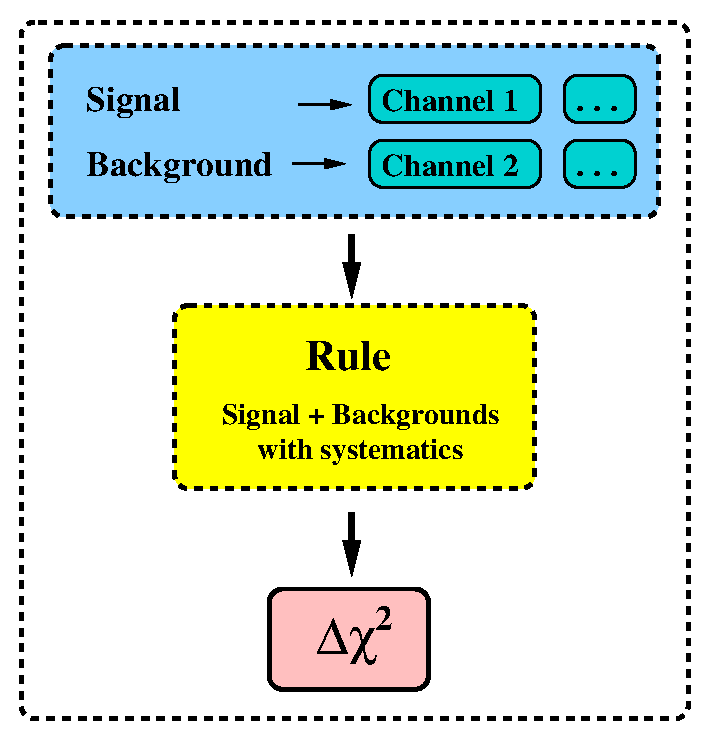
\includegraphics[width=8cm]{SignalBackground}
\end{center}
\caption{\label{fig:rule} General concept of a ``rule''.}
\end{figure}

\begin{figure}[t]
\begin{center}
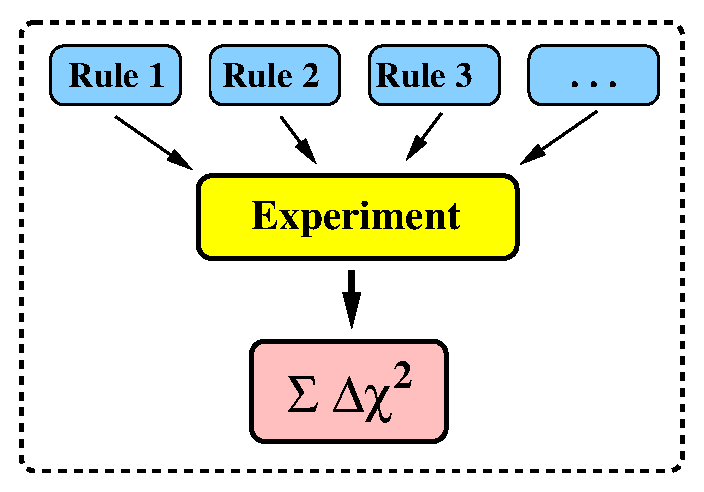
\includegraphics[width=9cm]{Rules}
\end{center}
\caption{\label{fig:experiment} General concept of an ``experiment''.}
\end{figure}

The channels are the building blocks for the so-called ``rules''.
\index{norm}{Rule} In general, a rule consists of one or more ``signal'' and ``background'' oscillation channels, which are normalized with efficiencies
(\cf, \figu{rule}). The event numbers from these channels are added {\em before} the $\Delta \chi^2$-value is calculated.\footnote{Note that
in this manual, the $\chi^2$ and $\Delta \chi^2$ are equal, since
for simulated data $\Delta \chi^2 = 0$ at the best-fit point. Thus, we
are using $\chi^2$ and $\Delta \chi^2$ as equal quantities.} In addition, each rule implements an {\em independent} systematics, such as signal and background normalization errors. Eventually, each rule gives a $\Delta \chi^2$-value, and the total $\Delta \chi^2$ of one experiment is obtained by adding the $\Delta \chi^2$'s of all rules (\cf, \figu{experiment}). 
 An example for a rule could look like this: We want to detect electron
  neutrino appearance (``signal''), where the overall efficiency for 
  quasi-elastics electron neutrino events is $0.4$. There is a fraction of 
  $0.01$ of all neutral current events which are mis-identified as 
  quasi-elastic electron neutrino events (``background''). The neutral 
  current fraction is only known within $10\%$ (``background uncertainty'') 
  and there is
an energy scale uncertainty of $100\,\mathrm{MeV}$ (``energy calibration error'').
All this systematics is independent of the other rules.  Thus, a rule connects the event rates to the calculation of a $\Delta \chi^2$ which properly includes systematical errors. The resulting $\Delta \chi^2$ is then the starting point for the oscillation physics analysis. Note again that
\begin{itemize}
\item
 Within each rule the event numbers are added.
\item
 Within each rule the systematics is treated independently from the other rules.
\item
 For each rule the $\Delta \chi^2$ is computed; the $\Delta \chi^2$'s from all rules are added.
\end{itemize}

Of course, an abstract experiment definition language can not simulate all possible types of experiments. As we have seen, there are several assumptions for source and detector. However, it turns out that \GLOBES\ can be applied to a large number of experiment types, such as conventional beams, superbeams, neutrino factories, $\beta$-Beams, and reactor experiments.

\section{A simple example for AEDL}

Experiments are in \GLOBES\ defined by the Abstract Experiment Definition Language (AEDL). The experiment definition is written into a text file using the AEDL syntax. Currently, a number of pre-defined experiment definition files are provided with \GLOBES , which have to be modified manually in order to define new experiments.  The application software then uses this text file to initialize the experiment, where other secondary files might read for source fluxes, cross sections \etc . In this section, we show the definition of a very simple neutrino factory in AEDL, where we do not go into details. In the next chapter, we will discuss each of the individual steps in detail.

The first line of every experiment definition file has to be
\begin{quote}
{\tt !\%GLoBES}
\end{quote}
in order not to confuse it with some other file format.
%
First, we instruct \GLOBES\ to use the built-in source flux for a neutrino factory
originating from stored $\mu^+$'s. This achieved by setting the {\tt @builtin} variable to $1$. Next, we specify the muon energy to be $50\,\mathrm{GeV}$ by the {\tt @parent\_energy} variable. We assume 
that there will be $5.33\cdot 10^{20}$ useful muon decays per year
and that this luminosity is available for $8$ years, \ie , a total number
of $ 4.264\cdot10^{21}$ muons is stored:
\begin{quote}
{\tt /* beam */}\\
{\tt flux(\#mu\_plus)<\\
\tb  @builtin = 1\\
\tb  @parent\_energy = 50.0\\
\tb  @stored\_muons = 5.33e+20\\
\tb  @time = 8.0\\
>}\\
\end{quote}
Note that we tell \GLOBES\ that we want to refer to this neutrino source later as as {\tt \#mu\_plus}. 
%
Let us now define a very simple detector with a target mass 
of $50\,\mathrm{kt}$ and $20$ energy bins between
$4\,\mathrm{GeV}$ and $50\,\mathrm{GeV}$: 
\begin{quote}
{\tt \$target\_mass = 50}\\
{\tt \$bins = 20}\\
{\tt \$emin = 4.0}\\
{\tt \$emax = 50.0}
\end{quote}
Then we specify the file which contains the cross sections we want to 
use:
\begin{quote}
{\tt /* cross section */}\\
{\tt cross(\#CC)<}\\
{\tt \tb @cross\_file = "XCC.dat"}\\
{\tt >}
\end{quote}
The command {\tt cross} tells the parser that a cross section environment
begins. It has the name {\tt \#CC}, which can later be used to refer 
to this specific environment, and thus to the file {\tt XCC.dat}. Note that each name begins with a leading {\tt \#}.
%
Of course, the baseline and matter profile have to be specified, too, where
we use an arbitrary matter density profile here:
\begin{quote}
{\tt /* baseline */}\\
{\tt \$profiletype = 3}\\
{\tt \$densitytab = \{3.5\}}\\
{\tt \$lengthtab = \{3000.0\}}\\
\end{quote}
The curly brackets used for the definition of {\tt \$densitytab} and
{\tt \$lengthtab} refer to a list of numbers. Here, the lists contain only
one element, because we only use one density layer: We initialize a baseline length of $3000 \, \mathrm{km}$ with a constant matter density of $3.5 \, \mathrm{g/cm^3}$. 
%
As another ingredient, we have to define the energy resolution function:
\begin{quote}
{\tt /* energy resolution */}\\
{\tt energy(\#MINOS)<}\\
{\tt \tb @type = 1}\\
{\tt \tb @sigma\_e = \{0.15,0.0,0.0\}}\\
{\tt >}
\end{quote}
The {\tt energy} command starts the energy environment, which has the name 
{\tt \#MINOS} here. Out of several possibilities, it uses algorithm one,
the simplest and fastest one. The actual energy resolution is specified
by the energy resolution variable, which is a list of three elements. Each 
element is one parameter of the general resolution function as defined in 
\eq~\ref{eq:sigma_e}.
%
Now we have all pieces to be able to define the appearance and the corresponding disappearance channel of a neutrino factory: 
$\nu_e\rightarrow\nu_\mu$  and $\bar\nu_\mu\rightarrow\bar\nu_\mu$ 
($\mu^+$ stored).
\begin{quote}
{\tt /* channels */}\\
{\tt channel(\#appearance)<}\\
{\tt \tb @channel = \#mu\_plus: +: electron: muon: \#CC: \#MINOS}\\
{\tt >}\\
{\tt channel(\#disappearance)<}\\
{\tt \tb @channel = \#mu\_plus: -: muon: muon: \#CC: \#MINOS}\\
{\tt >}
\end{quote}
The first element is the name of the flux, which we have defined above. 
The second element ``$\pm$'' determines whether 
neutrinos or anti-neutrinos are taken from the flux table (two different polarities allowed). The third position defines the initial flavor,
and the forth position the final flavor, followed by the name of the cross
section and energy resolution function as defined before.
%
The last step is to encapsulate the channels into a rule:
\begin{quote}
{\tt /* rules */}\\
{\tt rule(\#rule1)<}\\
{\tt \tb @signal = 0.45 @ \#appearance}\\
{\tt \tb @signalerror = 0.001 : 0.0001}\\
{\tt \tb @background = 1.0e-05 @ \#disappearance}\\
{\tt \tb @backgroundcenter = 1 : 0.0}\\
{\tt \tb @backgrounderror = 0.05 : 0.0001}\\
{\tt \tb @errordim\_sys\_on = 0}\\
{\tt \tb @errordim\_sys\_off = 2}\\
{\tt \tb @energy\_window = 4.0 : 50.0}\\
{\tt >}
\end{quote}
The {\tt @signal} refers to the ``signal'' in our experiment. We use the
above defined channel named {\tt \#appearance} with an constant overall
efficiency of $0.45$. The signal error variable has two components: 
The first one is the normalization error of the signal, here $0.1\%$. The second 
one refers to the energy calibration error of the signal, which is defined 
in \Sec~\ref{sec:energy}. The background variable
specifies the composition of the beam background. In this (simplified) case, we
use the fraction $1\cdot 10^{-5}$ of the channel named {\tt \#disappearance}, \ie , the muon neutrinos with a mis-identified charge. The background center variable allows to rescale the total background contribution from all background components
simultaneously. It is only useful if there is more than one background component, otherwise it is usually $1$. The background error variable is defined such as the signal error variable, \ie\ we have a $5\%$ background uncertainty and a very small energy calibration error. The ``error dimension variable'' {\tt @errordim\_sys\_X} selects how the systematical errors are treated (\cf, \Tab~\ref{tab:error_dim}). 

The here defined experiment represents a first simplified version of a neutrino factory experiment. It still lacks the correct energy dependence of the efficiencies, the antineutrino disappearance channel, and the channels and rules for the symmetric operation with $\mu^-$ stored. However, it may serve as a simple, introductory example. In the next chapter, we will demonstrate that the AEDL is much more powerful than illustrated here.


%%%%%%%%%%%%%%%%%%%%%%%%%%%%%%%%%%%%%%%%%%%%%%%%%%%%%%%%%%%%%%%%%%%%%%%%
\section{Introduction to the syntax of AEDL}
\label{sec:syntax}

We now give a short introduction to the syntax of AEDL.
 The first eight characters have to be {\tt \%!GLoBES}
in order to avoid parsing megabytes of chunk
 and producing thousands of error messages. 
%
Comments can be used such as in C:
\begin{quote}
{\tt /* This starts a comment\\
 and here the comment ends */
}
\end{quote}
There are pre-defined variables which all start with {\tt \$}. Their range
is also checked. For example,  {\tt 
\$bins} can be only between $0$ and $500$.\footnote{The upper limit is 
only there for safety reasons, the memory is allocated dynamically.} If one uses a {\tt float} quantity where  an {\tt int} is expected, the {\tt float} will be converted to an {\tt int} in the same way as in C.  For example, we have scalar variables
\begin{quote}
{\tt
\$bins = 10\\
\$baseline = 1200.0
}
\end{quote}
and simple lists
\begin{quote}
{\tt
\$densitytab=\{1.0,2.2343,3.3432\} 
}
\end{quote}
%
Since there are often groups of data which we want to refer to later,
environments can be used. This is illustrated 
with the channel definition part:
\begin{quote}
{\tt channel(\#ch1)<\\
\tb  $\ldots$\\
>
}
\end{quote}
The first part is the type of environment, which is {\tt channel} here. 
There are the following types of environment in AEDL:
\begin{quote}
{\tt flux\\
cross\\
channel\\
energy\\
rule
}
\end{quote}
Besides the environment type, there is a user-defined name 
beginning with {\tt \#}
in the above example: {\tt \#ch1}. It can be used later to refer to the 
channel defined in {\tt <$\ldots$>}. Those names are so-called 
``automatic variables'' and have to start with {\tt \#}. Note that these names have to be unique and can only be refered to after their definition.
However, similar to C, one can give a declaration without definition before:
\begin{quote}
{\tt    channel(\#ch2)<>}
\end{quote}
Now one can refer to the name {\tt \#ch2}, while the actual channel definition comes later. The internal representation of this automatic
variable is a number, which obtains its value from a counter for each type of environment. For example, for {\tt channel} the counter is {\tt numofchannels}. The counter keeps track of how many different names 
there are for one type of environment, which means that it counts the number of channels, rules, energy resolution functions \etc . Thus, the automatic
variables are numbered in the order of their definition, and the number
can later be used to refer to them in the C code (from $0$ to {\tt numof...}$-1$). In order to facilitate the the mapping from names in AEDL to indices
in C there are two functions \GLB{NameToValue} and \GLB{ValueToName} which
make this transition (see \Sec~\ref{sec:aedl_names}, 
page~\pageref{sec:aedl_names}).


Within each environment type, there are several 
variables beginning with {\tt @}, which can only be used within the 
appropriate type of environment. In many cases, 
they have a special syntax, such as {\tt @channel}.          

\index{aedl}{NEXT@{\tt \#NEXT\#}}
If you want to have several experiments in one file, separate the different
 experiments by 
\begin{quote}
{\tt    \#NEXT\#}
\end{quote}
This command resets the counters for channels, rules, fluxes, cross section 
and energy resolution environments. All variables have their scope limited 
by either {\tt \%!GLoBES, \#NEXT\#} or {\tt EOF}.  This allows 
a consistent treatment of various experiments in one file.

\index{aedl}{inlcude@{\tt include}}
As another feature of AEDL one can use include files with the {\tt include} command. Includes can be nested up to {\tt MAX\_INCLUSION\_DEPTH}, which is currently set to $10$. Error reporting works 
 for nested includes, too. The included file is not required to begin 
 with {\tt \%!GLoBES} to facilitate cut and paste:
\begin{quote}
{\tt include "./file\_1"}
\end{quote}
With this include mechanism, one can use constructions such as 
\begin{quote}
{\tt    include  "NuFact.gls"\\
        \#NEXT\#\\
        include   "JHFHK.gls"
}
\end{quote}
in order to initialize a combined analysis of the experiments defined in the files {\tt NuFact.gls} and {\tt JHFHK.gls}. Note that one has 
to use quotation marks for filenames in \AEDL.\index{norm}{File names}
Even if one uses the
automatic variable {\tt \#CC} in both experiments, 
but the cross section data are different (for example, because of different target nuclei), the correct 
cross section data will be applied to each of the experiments. 
Note that, alternatively, one can 
also load both files successively by two separate calls of 
\GLB{InitExperiment}. 

Furthermore, one can define constants such as
\begin{quote}
{\tt
Pi = 3.141
}
\end{quote}
These constants can not only be defined within one \AEDL\ file, but also
by the calling C program, which allows to use a simple but powerful variable
substitution mechanism as described in~\Sec~\ref{sec:aedlparams}.
\index{norm}{AEDL@\AEDL!external parameters}

In addition, some simple algebraic manipulations are possible, such as
\begin{quote}
{\tt
Pi+1\\
\verb+Pi^2+\\
sin(Pi/2)\\
}
\end{quote}
The following mathematical functions from {\tt <math.h>} are available: 
{\tt sin}, {\tt cos}, {\tt tan}, {\tt asin}, {\tt acos}, {\tt atan}, 
{\tt log}, {\tt log10}, {\tt exp}, {\tt sqrt}.
\index{aedl}{sin@{\tt sin}}
\index{aedl}{cos@{\tt cos}}
\index{aedl}{tan@{\tt tan}}
\index{aedl}{asin@{\tt asin}}
\index{aedl}{acos@{\tt acos}}
\index{aedl}{atan@{\tt atan}}
\index{aedl}{log@{\tt log}}
\index{aedl}{log10@{\tt log10}}
\index{aedl}{exp@{\tt exp}}
\index{aedl}{sqrt@{\tt sqrt}}



 
These functions can be used everywhere, where
otherwise only a scalar number would appear. However, they can not be
applied to lists, such as {\tt sin(\{1,2,3\})} will not work. 

Finally, note that a line feed character \verb+\n+ is necessary at
 the end of the input -- alternatively you can put a comment at the end.


%%%%%%%%%%%%%%%%%%%%%%%%%%%%%%%%%%%%%%%%%%%%%%%%%%%%%%%%%%%%%%%%%%%%%%%
\chapter{Experiment definition with AEDL}

In this chapter, we give a detailed definition of the AEDL features. We also show the underlying mathematical concepts, where applicable. We do not exactly follow the separation of source, oscillation, and detection properties, since most issues more or less involve the detection. Instead,
we illustrate many of the features of the \GLOBES\ simulation successively
in the logical order of their definition, and demonstrate how they translate into AEDL .

%%%%%%%%%%%%%%%%%%%%%%%%%%%%%%%%%%%%%%%%%%%%%%%%%%%%%%%%%%%%%%%%%%%%%%%%
\section{Source properties and integrated luminosity}
\label{sec:source}

As we have disussed before, \GLOBES\ can only deal with point sources. Thus,  it is not possible to study effects from the finite size of the neutrino production region, such as in the sun or in reactor experiments with many
neutrino sources (\eg, KamLAND). Therefore, a neutrino source in \GLOBES\ can, in general, be characterized by the flux spectrum for each neutrino flavor, the CP sign (neutrinos or antineutrinos), and the total luminosity
of the source.

Before we come to the definition of the source properties, let us discuss
the total integrated luminosity of the experiment. In \GLOBES , the total number of events is in general proportional to the product of
\begin{equation}
\mathrm{Fid.~detector~mass}\,\left[\mathrm{kt/t}\right]\times 
\mathrm{Running~time} \,\left[\mathrm{yr}\right]\times\left\{ \begin{array}{c}
\mathrm{Source~power}\,\left[\mathrm{MW/GW}\right]\\
\mathrm{Useful~muon~decays}\,\left[\mathrm{yr}^{-1}\right]
\end{array}\right.\,.
\end{equation}
Thus, the source power corresponds to either the amount of energy produced per time frame in the target (such as for nuclear reactors or sources based on pion decay), or the useful muon decays per time frame (neutrino factories). In addition, the definition of the source power makes only sense together with the flux normalization, the running time, and fiducial detector mass in order to define the total integrated luminosity. Therefore, one can, in principle, use arbitrary units for these components as long as their product gives the wanted neutrino flux. However, it is
recommended to use normalizations such that the source power units are $\mathrm{MW}$ for a proton-based beam, and $\mathrm{GW}_\mathrm{thermal}$ for a reactor experiment. Correspondingly, the detector mass units should be kilotons for a proton-based beam, and tons for a reactor experiment. In any case it is a good
idea to document the choices made by the user by corresponding comments
in \AEDL.

\index{aedl}{target mass@{\tt \$target\_mass}}
The quantity which can be used to scale the overall integrated luminosity of an experiment, is the fiducial detector mass. For example,
\begin{quote}
{\tt \$target\_mass = 50.0 }
\end{quote}
defines a $50 \, \mathrm{kt}$ detector for a neutrino factory.

\index{aedl}{{\tt flux}!time@{\tt "@time}}
There are two principal ways to initialize a neutrino flux: 
Either one can use 
a built-in source, or one can provide a file. In both cases,
a flux is defined by the environment {\tt flux}, such as
\index{aedl}{{\tt flux}}
\begin{quote}
  {\tt flux(\#name)<\\
\tb $\ldots$\\
\tb @time = 8.0 \\
>}
\end{quote}
with a running time of $8$ years. Note that the running time is used within
the {\tt flux} environment. This feature can be used to load the neutrino and antineutrino fluxes separately, in order to combine them with different
running times within one experiment. The name of the flux {\tt \#name} will later be refered to in the channel definitions.

For a built-in neutrino source, one has to specify which
built-in spectrum has to be used, as well as its parameters. The software
will then automatically calculate the neutrino spectrum. Note that in this
case, there is no degree of freedom in the choice of the source units.
Currently, two built-in fluxes are available: $\mu^+$-decay ({\tt @builtin = 1}) and $\mu^-$-decay ({\tt @builtin = 2}). In these cases, the muon energy (enery of the parent particle) has to be specified together with the number of useful decays  per year. Thus, an example to set up a neutrino factory flux is
\index{aedl}{{\tt flux}!builtin@{\tt "@builtin}}
\index{aedl}{{\tt flux}!parent energy@{\tt "@parent\_energy}}
\index{aedl}{{\tt flux}!stored muons@{\tt "@stored\_muons}}
\begin{quote}
{\tt flux(\#mu\_plus)<\\
\tb  @builtin = 1\\
\tb  @parent\_energy = 50.0\\
\tb  @stored\_muons = 5.33e+20\\
\tb  @time = 8.0\\
>}
\end{quote}
%
\index{aedl}{{\tt flux}!power@{\tt "@power}}
\index{aedl}{{\tt flux}!norm@{\tt "@norm}}
\index{aedl}{{\tt flux}!flux file@{\tt "@flux\_file}}
For a user-defined flux, one has to give it the file name:
\begin{quote}
{\tt flux(\#user)<}\\
{\tt \tb @flux\_file = "user\_file\_1.dat"\\
\tb @time = 2.0\\
\tb @power = 4.0\\
\tb @norm = 1e+8}\\
{\tt >}
\end{quote}
In this case, the {\tt @norm} variable is an overall normalization which defines a conversion factor from the fluxes in the file to the units in \GLOBES . In general, there are many ways to give the source power of a 
neutrino source, such as neutrinos per proton on target per area per time frame. Right now, each flux has its own normalization factor, which is
not always straightfoward to calculate. Often, one has to take into account
many things, such as the number of target particles per unit mass. 
In addition, the fluxes will be rescaled by $1/L^2$, which means that the
normalization must contain a factor $L_0^2$. Here $L_0$ is the distance from the source for which the flux is given to the actual neutrino production region. At the end, it is left to the user to ensure that the 
numbers in the flux file give, after the multiplication with {\tt @norm}, 
the proper numbers of produced neutrinos corresponding to the chosen target power {\tt @power}. Usually this adjustment of {\tt @norm} is performed by comparison with known energy spectra for a specific experiment.

\index{aedl}{{\tt flux}!flux file@{\tt "@flux\_file}}\index{norm}{Flux!file}
The software assumes that the given flux file has seven columns and
501 lines with equidistant energies. The format is:
\begin{quotation}
$ E\quad
\Phi_{\nu_e}\quad
\Phi_{\nu_\mu}\quad
\Phi_{\nu_\tau}\quad
\Phi_{\bar\nu_e}\quad
\Phi_{\bar\nu_\mu}\quad
\Phi_{\bar\nu_\tau}$
\end{quotation}
In order to access fluxes at arbitrary energies, linear interpolation 
is used by the software. In general, it is advisable to provide the flux between {\tt \$sampling\_min} and {\tt \$sampling\_max} (\cf, \Sec~\ref{sec:energy}), since these values are used by the software. However, if the energy leaves the range of values given in the file, zero is returned.
The the columns for the fluxes for unused flavours have to be filled all the 
same,\eg\ with zeros. 

The flux files accept one-line comments, which start
with {\tt \#} and end with the linefeed character `\verb+\n+', they are
not counted as a line and their content is discarded. This comments
are useful to provide meta information about the fluxes like units
or the origin of the information. This is also the default method
to point the user to the references he/she should to cite when using
a particular flux.\index{norm}{Flux!file!comments in}
\index{norm}{Referencing!flux data}

%%%%%%%%%%%%%%%%%%%%%%%%%%%%%%%%%%%%%%%%%%%%%%%%%%%%%%%%%%%%%%%%%%%%%
\section{Baseline and matter density profile}

The baseline and matter density profile determine, besides energy and
involved flavors, the neutrino oscillation physics at the experiment
description level. All of the neutrino oscillation parameters are defined at running time.

\index{aedl}{baseline@{\tt \$baseline}}
The baseline\index{norm}{Baseline} is given by
\begin{quote}
{\tt \$baseline = 3000.0 }
\end{quote}
Note that baseline lengths are always assumed to be in
kilometers.

\begin{table}[t!]
\begin{tabular}{|clp{7cm}|}
\hline
{\tt \$profiletype} & Additional variables & Description \\ 
\hline
$1$ & {\tt \$baseline} & Average density (constant) \\
$2$ & {\tt \$baseline}, {\tt \$densitysteps} & PREM profile with given number of equidistant steps \\
$3$ & {\tt \$lengthtab},  {\tt \$densitytab} & Arbitrary profile (table of layer thicknesses, table of densities) \\
\hline
\end{tabular}
\caption{\label{tab:profiletypes} Different matter density profiles which can be used with \GLOBES .}
\end{table}

\index{aedl}{profiletype@{\tt \$profiletype}}
\index{aedl}{densitysteps@{\tt \$densitysteps}}
\index{aedl}{lengthtab@{\tt \$lengthtab}}
\index{aedl}{densitytab@{\tt \$densitytab}}

Furthermore, the matter density profile along the baseline
has to be specified. The simplest matter density profile is a constant matter density profile with the average matter density from the PREM~\cite{Stacey} onion shell model of the earth\index{norm}{PREM| \see{Matter density}}
\index{norm}{Matter density!of the earth}:
\begin{quote}
{\tt \$profiletype=1 }
\end{quote}
%
If your using this option please cite reference~\cite{Stacey}\index{norm}{Referencing!matter profile data}.

For a better approximation of the realistic earth matter density profile, one can use an arbitrary number of equidistant steps of the PREM profile:
\begin{quote}
{\tt \$profiletype=2 } \\
{\tt \$densitysteps=20 }
\end{quote}
Note that the value of {\tt \$densitysteps} is time-critical, since the
computation time of oscillation probabilities is directly 
proportional to the number of layers.
%
As a  third possibility, one can specify the matter density profile 
manually with a list of thicknesses and densities of the matter density layers. This example uses two density steps with two different densities:
\begin{quote}
{\tt \$profiletype=3 } \\
{\tt \$densitytab=\{2.8, 3.5\}}\\
{\tt \$lengthtab=\{1000.0, 2000.0\}}
\end{quote}
It is important that both lists have the same length and that the  thicknesses given in  {\tt \$lengthtab} add up to the length of
the baseline, which does not have to be explicitely specified anymore. In addition, matter densities are always given in $g/cm^3$.
%
This approach can also be used for a constant matter density profile with
a specific matter density:
\begin{quote}
{\tt \$profiletype=3 } \\
{\tt \$densitytab=\{3.5\}}\\
{\tt \$lengthtab=\{3000.0\}}
\end{quote}
The possible options for matter density profiles are summarized in \Tab~\ref{tab:profiletypes}.

%%%%%%%%%%%%%%%%%%%%%%%%%%%%%%%%%%%%%%%%%%%%%%%%%%%%%%%%%%%%%%%%%%%%%%%%%%%%%

\section{Cross sections}
\label{sec:cross_section}

Cross sections\index{norm}{Cross section} will later be used as part of the 
channel definition (see \Sec~\ref{sec:channel}). Similar to the source 
fluxes, they are provided by the user as a data file:
\index{aedl}{{\tt cross}}
\index{aedl}{{\tt cross}!cross file@{\tt  "@cross\_file}}
\begin{quote}
{\tt cross(\#name)<}\\
{\tt \tb @cross\_file ="user\_file\_1.dat"}\\
{\tt >}
\end{quote}  
This cross section can later be refered to by {\tt \#name}.

Cross sections are in \GLOBES\ given as differential cross section per energy:
\begin{equation}
\hat\sigma(E)=\sigma(E)/E\,\left[ 10^{-38}\,
\frac{\mathrm{cm}^2}{\mathrm{GeV}^2} \right]
\end{equation}
The software assumes that the cross section files are text files with 
seven columns and $1001$ lines of the form
\index{norm}{Cross section!file}
\index{aedl}{{\tt cross}!cross file@{\tt  "@cross\_file}}
\begin{quotation}
$\mathrm{log}_{10} E\quad
\hat\sigma_{\nu_e}\quad
\hat\sigma_{\nu_\mu}\quad
\hat\sigma_{\nu_\tau}\quad
\hat\sigma_{\bar\nu_e}\quad
\hat\sigma_{\bar\nu_\mu}\quad
\hat\sigma_{\bar\nu_\tau}$
\end{quotation}
Here the logarithms of the energy values have to be equidistant. For 
arbitrary energies, linear interpolation is used. If the energy leaves the
range of values given in the file, $0.0$ will be assumed. In general, it is advisable to provide the cross sections in the range between {\tt \$sampling\_min} and {\tt \$sampling\_max} (\cf, \Sec~\ref{sec:energy}).
Unused cross sections have to be filled with zeros, and can not
 be just omitted.

Like the flux files, the cross section files 
accept one-line comments, which start
with {\tt \#} and end with the linefeed character `\verb+\n+', they are
not counted as a line and their content is discarded. This comments
are useful to provide meta information about the cross sections like units
or the origin of the information. This is also the default method
to point the user to the references he/she should to cite when using
a particular cross section.\index{norm}{Cross section!file!comments in}
\index{norm}{Referencing!cross section data}

\section{Oscillation channels}
\label{sec:channel}

\index{aedl}{{\tt channel}|(}
Channels\index{norm}{Channel} in \GLOBES\ represent an intermediate level 
between the pure oscillation physics given by the oscillation probability
$P_{\alpha\beta}$, and the total event rates composed of signal and 
background. A channel describes the path from one
initial neutrino flavor in the source to the event rates in the detector for one specific interaction type (IT) and final flavor.  
Therefore, a channel contains the description of the 
initial neutrino flavor, its CP eigenvalue 
(neutrino or antineutrino)\footnote{Currently \GLOBES\ does not support lepton
number violating transitions, \ie\ no transitions from neutrino to 
antineutrino (or vice versa) are considered.}, 
the detected neutrino flavor, the interaction cross sections for the chosen interaction type, and the energy resolution function of the detector.

Before we come to the definition of the channel in AEDL, we introduce the general concept for the calculation of event rates. The first step is to
compute the number of events for each IT in the detector for each 
initial and final neutrino flavor and energy bin. The second step is to include the detector effects coming from the insufficient knowledge in the event reconstruction. These two steps combined lead to the differential event rate spectrum for each initial and final flavor and IT as seen by the detector, which we call the ``channel''. In this section, we focus on the
 first step, \ie , we discuss the definition of the energy resolution function in the next section, since this is a rather comprehensive issue.

The differential event rate for each channel is given by
%%%%%%%%%%%%%%%%%%%%%%%%%%%%%%%%%%%
\begin{eqnarray}
\label{eq:master_event}
\frac{dn_{\beta}^{\text{IT}}}{dE'}=&&N\,\int\limits_0^\infty \int\limits_0^\infty dE\,d\hat{E}\quad
\underbrace{\Phi_{\alpha} (E)}_{\mathrm{Production}} \times \nonumber\\
&&\underbrace{\frac{1}{L^2} P_{(\alpha\rightarrow\beta)}(E,L,\rho;\theta_{23},
\theta_{12},\theta_{13},
\Delta m^2_{31},\Delta m^2_{21},\deltacp)}_{\mathrm{Propagation}}
\times \nonumber \\ &&\underbrace{\sigma^{\text{IT}}_f(E)
k_f^{\text{IT}}(E-\hat{E})}_{\mathrm{Interaction}} \times \nonumber \\
&&\underbrace{ T_f(\hat{E}) V_f(\hat{E}-E')}_{\mathrm{Detection}}\,,
\end{eqnarray}
%%%%%%%%%%%%%%%%%%%%%%%%%%%%%%%%%%%
where $\alpha$ is the initial flavor of the neutrino, 
$\beta$ is the final flavor, $\Phi_{\alpha} (E)$ is the flux of the 
initial flavor at the
source, $L$ is the baseline length, $N$ is a normalization factor, and 
$\rho$ is the matter density. The energies in this formula are given as follows:
\begin{itemize}
\item
 $E$ is the incident neutrino energy, \ie, the actual energy of the 
incoming neutrino (which is not directly accessible to the experiment)
\item
 $\hat{E}$ is the energy of the secondary particle
\item
 $E'$ is the reconstructed neutrino energy, \ie, the measured
neutrino energy as obtained from the experiment
\end{itemize}
The interaction term is composed of 
two factors, which are the total cross section 
$\sigma^{\text{IT}}_\beta(E)$ for the flavor $f$ and
the interaction type IT, and the energy distribution of the 
secondary particle $k_\beta^{\text{IT}}(E-\hat{E})$.
The detector properties are 
modeled by the threshold function $T_\beta(\hat{E})$, coming from the the 
limited resolution or the cuts in the analysis, and the energy resolution 
function $V_\beta(\hat{E}-E')$ of the secondary particle. 

Since it is a lot of effort to solve this double integral numerically,
we split up the two integrations. First, we evaluate the integral over
$\hat{E}$, where the only terms containing $\hat{E}$ are
$k_\beta^{\text{IT}}(E-\hat{E})$,  $ T_\beta(\hat{E})$, and 
$ V_\beta(\hat{E}-E')$. We define:
\begin{eqnarray}
\label{eq:e_res} 
R_\beta^{\text{IT}}(E,E')\,\epsilon_\beta^{\text{IT}}(E')
 \equiv
\int\limits_0^\infty d\hat{E} \quad T_\beta(\hat{E})\,k_\beta^{\text{IT}}(E-\hat{E})
\,V_\beta(\hat{E}-E')\,. 
\end{eqnarray}
Thus, $R_\beta^{\text{IT}}(E,E')$ describes the energy response of 
the detector, \ie , a neutrino with a (true) energy $E$ is reconstructed
with an energy between $E'$ and $E'+dE'$ with a probability
$R_\beta^{\text{IT}}(E,E') dE'$. The function $R(E,E')$ is also often called ``energy resolution function''. Actually, its internal representation
in the software is a smearing matrix\index{norm}{Energy!resolution}\index{norm}{Smear matrix}. The function $\epsilon_\beta^{\text{IT}}(E')$ will later be refered to as ``post-smearing efficiencies'', since it will allow us to define cuts and threshold functions {\em after} the smearing is performed, \ie, as function of $E'$. The detailed definition and initialization of the energy resolution function is described in \Sec~\ref{sec:energy}.

Eventually, we can write down the number of events per bin $i$ \index{norm}{Bin} and channel $c$ as
\begin{equation}
\label{eq:channel}
n_i^c=\int_{E_i-\Delta E_i/2}^{E_i+\Delta E_i/2} dE' \quad
\frac{dn_{\beta}^{\text{IT}}}{dE'} (E') \,
\end{equation}
where $\Delta E_i$ is the bin size of the $i$th energy bin.
This means that one has to solve the integral
\begin{eqnarray}
\label{eq:events_bin}
n_i^c=N/L^2\,\int_{E_i-\Delta E_i/2}^{E_i+\Delta E_i/2} dE' 
\quad \int\limits_0^\infty dE \,\, \Phi^c(E)\,
P^c(E)\,
\sigma^c(E)\,
R^c(E,E')\,
\epsilon^c(E')\,.
\end{eqnarray} 
Note that the events are binned according to their \emph{reconstructed} energy.

A simple channel definition in \GLOBES\ consists of the flux,
the CP-sign of the initial state, the initial flavor, the final flavor,
the cross sections, and the energy resolution function. In order to refer to
flux, cross sections, and energy resolution functions, they have to be 
defined before with their {\tt \#name} in the respective environments. 
Thus, a simple definition of a channel\index{aedl}{{\tt channel}} is
\begin{quote}
{\tt channel(\#channel\_1)<\\
\tb @channel = \#flux : $+$: muon: muon: \#cross: \#energy\\
>}
\end{quote}
%
\index{norm}{Oscillation!switching off}
It is also possible to define a channel as no-oscillation by using the
prefix {\tt NOSC\_}\index{aedl}{{\tt channel}!{\tt NOSC\_}} 
in either the initial  flavour or 
the final flavour, like this
\begin{quote}
{\tt channel(\#channel\_1)<\\
\tb @channel = \#flux : $+$: NOSC\_muon: muon: \#cross: \#energy\\
>}
\end{quote}
%
In this case all diagonal probabilities $P_{\alpha\alpha}$ are unity, and all off-diagonal probablities  $P_{\alpha\beta}$ are zero. This is,
for instance, useful for
neutral current events, since these do not depend on any oscillation 
parameters\footnote{At least in the absence of sterile neutrinos}. The channels
marked as {\tt NOSC\_} are already computed by \GLB{SetRates}
and do not have to be recomputed in the subsequent fit (which calls the undocumented function \GLB{SetNewRates}).
Therefore this feature can be used to speed up the rate 
computation considerably, especially in cases where a large set
of channels exist which are only used for the computation of backgrounds.
Usually it is an excellent approximation to treat backgrounds as if they
were not affected by oscillations\footnote{In case, the backgrounds have
a sizeable dependence on the oscillation parameters they carry information
on the oscillation parameters and are therefore more like a signal.}.

Note that the energy environment will be described in the next section. 
In addition, one can define pre- and post-smearing effects together
with the channels, which will also be introduced together with the
energy resolution function in the next section.
\index{aedl}{{\tt channel}|)}

%%%%%%%%%%%%%%%%%%%%%%%%%%%%%%%%%%%%%%%%%%%%%%%%%%%%%%%
\section{Energy resolution function}
\label{sec:energy}

\index{aedl}{{\tt energy}|(}
\index{norm}{Energy!resolution|(}
The definition and implementation of the energy resolution function is 
rather sophisticated in \GLOBES . In particular, the choice of the 
proper parameters depends on the experiment and the frequencies of the
 involved neutrino oscillations. This choice also greatly influences the
speed of the calculation.

In this section, we first discuss the principles of the energy smearing, where it is assumed that the reader is familiar with \Sec~\ref{sec:channel}. Then we introduce an automatic energy smearing algorithm, which is fairly simple to understand and applicable to most beam-based experiments. 
In most cases, the reader may want to continue to the next section after reading these two subsections. In the third subsection, we describe a more elaborate (and slower) smearing algorithm, which can be used together with rather fast neutrino oscillations compared to the bin size, such as for
(solar) reactor experiments to avoid aliasing effects. Eventually, we show how one can use a manual smearing matrix instead of using one of the implemented algorithms.

\subsection{Introduction and principles}

The energy resolution function $R^c(E,E')$ has been already introduced in 
\Sec~\ref{sec:channel}, where a definition
has been given in \eq~(\ref{eq:e_res}). Instead of using
 \eq~(\ref{eq:e_res}) directly, we apply a slightly different
definition of the post-smearing efficiencies $\epsilon(E')$. 
In general, $\epsilon(E')$ has to be
determined by means of a Monte Carlo simulation of the experiment. 
This usually involves a binning of the simulated events in the 
reconstructed energy $E'$. Therefore, one simplify \eq~(\ref{eq:events_bin}) by
\begin{equation}
\label{eq:post_smearing}
\int_{E_i-\Delta E_i/2}^{E_i+\Delta E_i/2} dE' \, R^c(E,E') \, \epsilon^c(E')
 \simeq \hat\epsilon_i^c \cdot \int_{E_i-\Delta E_i/2}^{E_i+\Delta E_i/2} dE' 
\quad R^c(E,E')\,.
\end{equation}
Here the  $\hat\epsilon_i^c$ are the 
binned ``post-smearing'' efficiencies, which will be set within the corresponding {\tt channel} environment (see below).
From \eq~(\ref{eq:events_bin}) it is obvious that the integration with respect to the reconstructed energy $E'$ can be
performed independently of the oscillation parameters. We define
the ``bin kernel'' $K_i^c$ for the $i$th bin as
\begin{equation}
\label{eq:kernel}
K_i^c(E) \equiv \int_{E_i-\Delta E_i/2}^{E_i+\Delta E_i/2} dE' 
\quad R^c(E,E')\,.
\end{equation}
With this definition, \eq~(\ref{eq:events_bin}) can be re-written as
\begin{equation}
\label{eq:simple_int}
n_i^c=N/L^2 \,
\hat\epsilon_i^c \, \int\limits_0^\infty dE\quad  \underbrace{\Phi^c(E)\,
P^c(E)\,
\sigma^c(E) \, K_i^c(E)\,}_{f(E)}. 
\end{equation}

There is no principle reason why one should not evaluate this integral directly by the usual numerical methods. However, it turns out that this 
is very slow in many cases. Therefore, we will introduce two different approximation schemes for different applications in the next two subsections.
In either case, the integrand in \eq~(\ref{eq:simple_int}) has to be evaluated at fixed ``sampling points''. These sampling points have to directly 
or indirectly be defined by the user.

\begin{figure}[t!]
\begin{center}
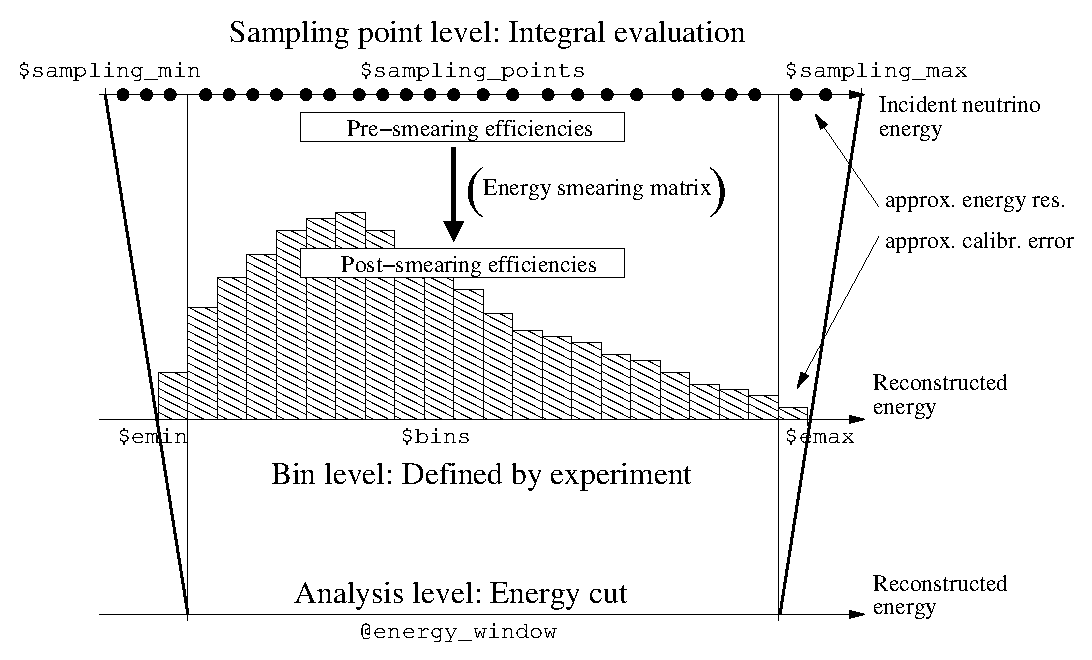
\includegraphics[width=15cm]{energies}
\end{center}
\caption{\label{fig:energies} The different evaluation levels for the energy smearing in \GLOBES .}
\end{figure}

Before we come to the calculation algorithms, it is useful to understand
the general evaluation algorithm. As it is illustrated in \figu{energies}, 
\GLOBES\ uses several levels with respect to the energy ranges:
\begin{description}
\item[Sampling point level]
 This level is used internally to evaluate the integrand in \eq~(\ref{eq:simple_int}) at all sampling points. The energy scale is the actual incident neutrino energy $E$. 
For a manual definition of the sampling points, use
\index{aedl}{sampling points@{\tt \$sampling\_points}}
\index{aedl}{sampling min@{\tt \$sampling\_min}}
\index{aedl}{sampling max@{\tt \$sampling\_max}}
\begin{quote}
{\tt
\$sampling\_points = 20\\
\$sampling\_min =          4.0\\
\$sampling\_max =         50.0
}
\end{quote}
for equidistant sampling points. If no values are given for these variables
they are assumed to be equal to their corresponding counter part at bin level,
\ie\ \verb+$sampling_points = $bins+, \verb+$sampling_min = $emin+ and
\verb+$sampling_max = $emax+.


Arbitrarily spaced sampling points can 
be specified with 
{\tt \$sampling\_stepsize}\index{aedl}{sampling stepsize@{\tt \$sampling\_stepsize}}
\begin{quote}
{\tt
\$sampling\_stepsize=\{1.0,2.0,3.0,4.0,5.0,...\}
}
\end{quote}
The choice of the sampling point configuration strongly depends on the 
experiment and required accuracy. Ideally the integrand 
of~\eq~\ref{eq:simple_int} is zero outside the sampling range, if this cannot
be achieved it is usually sufficient that the sampling range is by about
three times the energy resolution\footnote{evaluated at {\tt \$emin} and
{\tt \$emax} respectively} larger than the bin range. 
The spacing of the sampling points should be somewhat smaller (a factor 
$\simeq 2$ usually is more than ebough) than the 
finest details of the integrand.



\item[Bin level] This level is determined by the experiment and its analysis. 
Note that energy
bin sizes much smaller than the energy resolution will not improve the results. The energy bin range and the number of energy bins do always have to be specified. For the case of large values of the integrand in \eq~(\ref{eq:simple_int}) at the energy range limits, it is recommended to exceed the analysis energy window by about three times the energy calibration error in order 
to avoid cutoff effects.

In order to define a range between $E_\mathrm{min}$
and $E_\mathrm{max}$ divided by a certain number of equidistant bins,
use
\index{aedl}{emax@{\tt \$emax}}
\index{aedl}{emin@{\tt \$emin}}
\index{aedl}{bins@{\tt \$bins}}
\begin{quote}
{\tt
\$emin = 4.0\\
\$emax = 50.0\\
\$bins = 20
}
\end{quote}
For arbitrary bins, use $E_\mathrm{min}$
and $E_\mathrm{max}$ and the size of each bin  $\Delta E_i$:
\begin{quote}
{\tt
\$emin = 4.0\\
\$emax = 50.0\\
\$binsize = \{  15.0 , 5.0 , 20.0, 6.0 \} 
}
\end{quote}
\index{aedl}{binsize@{\tt \$binsize}}
The number of bins will be automatically computed by \GLOBES . Note that the
bin sizes have to add up to the energy range {\tt \$emax}-{\tt \$emin}.

The choices at bin level are mainly determined by optimizing the
performance of the experiment.

\item[Analysis level]
On the analysis level, an energy window can be defined within each rule. For
details, see next chapter.
\end{description}

In general, the energy smearing happens between the sampling point and bin levels, which means that the energy smearing matrix will have {\tt \$sampling\_points} columns and {\tt \$bins} rows. 

As illustrated in the figure, an interesting feature in combination with the
channels are pre- and post-smearing effects. Pre-smearing effects are taken into account on the sampling point level, and post-smearing effects on the bin level. Examples for these effects are energy 
dependent efficiencies and (non-beam) backgrounds. Efficiencies are multiplicative factors, whereas backgrounds are added to the event rates. These components can be introduced before or after the integration in \eq~(\ref{eq:simple_int}) is done. 
%
\index{aedl}{{\tt channel}!pre smearing efficiencies@{\tt 
"@pre\_smearing\_efficiencies}}
\index{aedl}{{\tt channel}!pre smearing background@{\tt 
"@pre\_smearing\_background}}
\index{aedl}{{\tt channel}!post smearing efficiencies@{\tt 
"@post\_smearing\_efficiencies}}
\index{aedl}{{\tt channel}!post smearing background@{\tt 
"@post\_smearing\_background}}
%
If they are introduced before, 
we call them
{\tt @pre\_smearing\_efficiencies} or {\tt @pre\_smearing\_background}. 
If they are introduced after, we call them {\tt @post\_smearing\_efficiencies} or {\tt @post\_smearing\_background}.
Note that pre-smearing components are always a function of the incident neutrino energy $E$. Thus, there have to be as  many elements as there are sampling points. 
Examples for pre-smearing quantities are non-beam backgrounds, such as from geophysical neutrinos. The post-smearing components are always a function of the reconstructed neutrino energy $E'$, such as the post-smearing efficiencies $\epsilon_\beta^{\text{IT}}(E')$ in \eq~(\ref{eq:e_res}). Examples for post-smearing efficiencies are cuts and detection threshold functions. All post-smearing components have to have as 
many elements as there are energy bins. Efficiencies are multiplicative 
and their default value is $1$, whereas backgrounds are additive and their default value is $0$. Thus, a more elaborate channel can be defined as
\begin{quote}
{\tt channel(\#channel\_1)<\\
\tb @channel = \#flux : $+$: muon: muon: \#cross: \#energy\\
\tb @pre\_smearing\_background = \{1,2,3,4,5,6,7,8,9,10\}\\
\tb @post\_smearing\_efficiencies = \{0.1,0.2,0.3,0.4,0.5\}\\
>}
\end{quote}
%
\index{aedl}{{\tt channel}!pre smearing efficiencies@{\tt 
"@pre\_smearing\_efficiencies}}
\index{aedl}{{\tt channel}!pre smearing background@{\tt 
"@pre\_smearing\_background}}
\index{aedl}{{\tt channel}!post smearing efficiencies@{\tt 
"@post\_smearing\_efficiencies}}
\index{aedl}{{\tt channel}!post smearing background@{\tt 
"@post\_smearing\_background}}
%
This experiment uses $10$ sampling points and $5$ bins.

In the following subsections we will define the energy resolution function.
All energy resolution functions are defined within an {\tt energy} environment and can be refered to by {\tt \#name}.
\begin{quote}
  {\tt energy(\#name)<\\
\tb $\ldots$\\
>}
\end{quote}
The individual parameters of the environment will be defined below and depend on the algorithm used.

\subsection{Bin-based automatic energy smearing}

This algorithm is the simplest of the built-in algorithms for the evaluation
of \eq~(\ref{eq:simple_int}). It is applicable to most of the
experiments which can be simulated with \GLOBES .

The key idea is to use a ``flat'' model, \ie\ the integrand 
of~\eq~\ref{eq:simple_int}  is well approximated by being piecewise
constant in each sampling step. This is a good approximation as long as
\begin{itemize}
\item
 No details are lost, \ie\ the spacing of sampling points 
is smaller than the energy resolution.
\item
The edges are treated correctly.
\item
 The neutrino oscillations are slow on a scale of the smapling point distance.
\end{itemize}
In this case, \eq~(\ref{eq:simple_int}) is reduced to
\begin{equation}
\label{eq:algo_one}
n_i^c=N/L^2 \, \sum_{j=1}^N \,  \Phi^c(E_j)\,
P^c(E_j)\,
\sigma^c(E_j)\,
K_i^c(E_j) \, \Delta E_j \,.
\end{equation}
The advantages of this algorithm are obvious: All factors
independent of the oscillation parameters have to be only evaluated once
at values of $E$ which are known in advance, which means that they can be put 
into a look-up table. In addition, the probability
has to be only evaluated at previously known values of the energy, which
makes it possible to compute the transition amplitudes for all channels
simultaneously. One assumption is that all involved factors are piece-wise
constant, \ie, they hardly change within each bin. This 
assumption seems to be very restrictive, which is however not quite correct.
First of all, if one analyzes simulated data (which are simulated with the same algorithm), the errors
will cancel between the simulated and fitted data. Second, and more important,
this algorithm is just a very basic integration routine\footnote{It is planed 
for to have something like a Gau\ss-Kronrod scheme as an alternative here.} and converges to
the true result for decreasing step size. Thus if the number of sampling
points is large enough this algorithm is very accurate. 
This algorithm is selected by
%
\index{aedl}{{\tt energy}!type@{\tt "@type}}
%
\begin{quote}
{\tt \tb @type = 1}
\end{quote}
within the {\tt \#energy} environment.
The computation of the bin kernel $K_i^c$ is performed
by \GLOBES. Thus, it requires that the number of bins
{\tt \$bins} and the minimum energy {\tt \$emin} and maximum energy {\tt \$emax} are given in case of equidistant bins.
%
\index{norm}{Energy!resolution}
\index{norm}{Energy!resolution function}
%
As far as the parameterization for the energy resolution function 
$R^c(E,E')$ in \eq~(\ref{eq:kernel}) is concerned, the algorithm uses
a Gau\ss ian
\begin{equation}
R^c(E,E')=\frac{1}{\sigma(E)\,\sqrt{2\pi}}\,e^{-\frac{(E-E')^2}{2\sigma^2(E)}} \, .
\end{equation} 
%
\index{aedl}{{\tt energy}!sigma function@{\tt "@sigma\_function}}
%
There are several energy resolution functions available, where by default
{\tt \#standard} is used:
\begin{quote}
{\tt \tb @sigma\_function = \#standard} 
\end{quote}
%
\index{aedl}{{\tt energy}!standard@{\tt \#standard}}
%
The energy resolution function {\tt \#standard} is defined by
\begin{equation}
\label{eq:sigma_e}
\sigma(E)=\alpha\cdot E + \beta \cdot \sqrt{E} +\gamma\, ,
\end{equation}
where the parameters $\alpha, \beta$ and $\gamma$ are provided by the user:
\begin{quote}
{\tt \tb @sigma\_e = \{0.15, 0.0, 0.0\}}
\end{quote}
Currently, another possible choice for {\tt @sigma\_function} is {\tt \#inverse\_beta},
%
\index{aedl}{{\tt energy}!inverse beta@{\tt \#inverse\_beta}}
%
which only uses the parameter $\alpha$. It is defined by
\begin{equation}
\sigma(E)= \left\{\begin{array}{cl}
 \alpha \cdot \sqrt{1000}^{-1}\,\sqrt{x-8\cdot10^{-4}}\,,&\mathrm{for}\,\, 
x>1.8\cdot10^{-3}\\
\alpha\cdot10^{-3} \,,&\mathrm{for}\,\, x \leq 1.8\cdot10^{-3}
\end{array} \right.
\end{equation}
The somewhat complicated form is due to the fact that inverse $\beta$-decay
has a neutrino threshold of $1.8\,\mathrm{MeV}$ and that a neutrino
at threshold already produces $\simeq 1\,\mathrm{MeV}$ visible energy in
the detector (for more details see \eg~\cite{Huber:2003pm}). 

In the actual implementation of the algorithm,  the sum in \eq~(\ref{eq:algo_one}) is only computed for the $E_j$'s where $K(E_j)$ 
is above a certain threshold, which is by default $10^{-7}$. 
This threshold is defined at the compiling time. 

Eventually,  a complete energy resolution definition of this 
algorithm is, for example,
\begin{quote}
{\tt energy(\#name)<\\
\tb @type = 1\\
\tb @sigma\_function = \#standard\\
\tb @sigma\_e = \{0.15 ,0.0 ,0.0\}\\
>
}
\end{quote}

\subsection{Low-pass filter}

In order to ensure that fast oscillating probabilities do not lead to 
aliasing,\index{norm}{Aliasing}
it is possible to impose a low-pass filter already during the calculation
of the probabilities itself. This filter is implemented has a highly
experimental feature called ``filter''\index{norm}{Filter}. 
The calculation of oscillation
probabilities is, in principle, a computation of phase differences. Restricting the maximum admissible size of those phase differences effectively filters
the high frequency component of the oscillation probability. This idea is
implemented according to
\begin{eqnarray}
\label{eq:filter_a}
P_{\alpha\beta}(E)&=&\sum_{ij}
U_{\alpha j} U^*_{\beta j} U^*_{\alpha i} U_{\beta i} 
e^{-i\Phi_{ij}}\times 
e^{ -\Phi_{ij}^2/\sigma_f(E)^2 }\,,
\end{eqnarray}
where $\Phi_{ij}:=\Delta m_{ij}^2 L/2E$ is the usual phase difference and
the last term is a Gau\ss ian filter with width $\sigma_f(E)$. Choosing
$\sigma_f(E):=\sigma_f^0 \cdot E$ ensures that this filter behaves 
approximately such as an energy resolution function with constant width 
$\sigma_e=\sqrt{2}/\sigma_f^0$, \ie\
\begin{equation}
\label{eq:filter_b}
\int d\tilde E\quad P(\tilde E) \frac{1}{\sigma_e\,\sqrt{2\pi}}\,
e^{-\frac{(E-\tilde E)^2}{2\sigma^2_e}}\,.
\end{equation}
The relationship between \eqs~\ref{eq:filter_a} and~\ref{eq:filter_b}
is not obvious and connected to the properties of $P_{\alpha\beta}$: 
see \Refs~\cite{Kiers:1996zj,Giunti:2003ax}. This feature works \emph{only} 
for vacuum and constant densities and is controlled
by the filer state variable. In addition, $\sigma_e$ is set by the filter value variable:
\index{aedl}{filter state@{\tt \$filter\_state}}
\index{aedl}{filter value@{\tt \$filter\_value}}
\begin{quote}
{\tt
\$filter\_state = 1\\
\$filter\_value = 2.0\\
}
\end{quote}
would switch the filter feature on and set the width to $2.0\,\mathrm{GeV}$.
The setting of {\tt \$filter\_state} is ignored whenever a density profile
with more than one layer is used. 

\index{aedl}{{\tt energy}!type@{\tt  "@type}}
With a type 1 ({\tt @type = 1}) energy resolution 
function, $\sigma_e$ adds on to the energy resolution function 
of the detector $\sigma_c(E)$ such as
\begin{equation}
\sigma_{\mathrm{eff}}(E)^2\simeq \sigma_e^2 + \sigma_c(E)^2\,.
\end{equation} 
Sometimes this behavior is unwanted, and therefore one can try to 
'subtract' the filtering from the energy resolution function by splitting 
the energy resolution function $\sigma(E)_{\mathrm{eff}}$ in
two parts by
\begin{equation}
\sigma_{\mathrm{eff}}(E)^2=\underbrace{\sigma_c(E)^2-\sigma_e^2}_
{\tilde\sigma^2_c(E)}+\sigma_e^2\,,
\end{equation}
where the truncated energy resolution function $\tilde\sigma_c(E)$ 
is used instead of $\sigma_c(E)$ in computing the
smearing data. Thus one obtains as effective energy resolution
\begin{equation}
\sigma_{\mathrm{eff}}(E)^2\simeq \sigma_c(E)^2\,.
\end{equation} 
This scheme is used by choosing as type for the energy resolution
\begin{quote}
{\tt
@type = 2
}
\end{quote}

\subsection{Manual energy smearing}

In some cases, one may use the output of a detector Monte Carlo simulation
directly. Then one can use ''manual'' energy smearing instead  of the
automatic energy smearing algorithms. 

The energy smearing matrix $K_{ij}$ has {\tt \$bins} rows and {\tt \$sampling\_points} columns, which are numbered from $0$ to {\tt \$bins}$-1$ or {\tt \$sampling\_points}$-1$. It is equivalent to the 
bin- and sampling-point-based kernel in \eq~(\ref{eq:kernel}):
\begin{equation}
K_{ij} = K_i^c(E) |_{E=E_j},
\label{equ:ematrix}
\end{equation}
where $E_j$ is the energy of the $j$th sampling point. In general, many of the entries in this matrix are zero, which means that it is convenient to evaluate the integrand in \eq~(\ref{eq:simple_int}) only at positions where
$K_{ij}$ is non-zero. The corresponding ``sampling range'' range of non-zero matrix entries  in $K_{ij}$ for the $i$th energy bin is defined to run from
column $k_l^i$ (``lower index'') to column $k_u^i$ (``upper index'').
An example for a smearing matrix is
\begin{equation}
K_{ij} =   \underbrace{ \left( \begin{array}{cccccccccc} 
a_{00} & a_{01} & a_{02} & a_{03} &  &  &  &  &  & \\
a_{10} & a_{11} & a_{12} & a_{13} & a_{14} &  &  &  &  &  \\
 & a_{21} & a_{22} & a_{23} & a_{24} & a_{25} &  &  &  &  \\
 &  & a_{32} & a_{33} & a_{34} & a_{35} & a_{36} &  &  &  \\
 &  &  & a_{43} & a_{44} & a_{45} & a_{46} & a_{47} &  &  \\
& & & \uparrow  & & \ddots & & \uparrow & & \\
& & & k_l^i & & & & k_u^i & & \\ 
\end{array}\right) }_{\mathtt{\$sampling\_points}  \, \, \mathrm{columns}} \quad \leftarrow \quad \footnotesize{\mathtt{\$bins} \, \, \mathrm{rows}} \, ,
\end{equation}
where the unshown entries are zero. Thus, the values of $K_{ij}$ have to be specified between $k_l^i$ and $k_u^i$ in the form $\{ k_l^i,k_u^i, K_{i \, k_l^i}, K_{i k_l^i+1} , \hdots , K_{i k_u^i} \}$:
\index{aedl}{{\tt energy}!energy@{\tt "@energy}}
\begin{quote}
{\tt 
energy(\#name)<\\
\tb @energy =   \{0,2, 0.8634265, 0.0682827,     4e-06\}:\\
\tb\tb \{0,4, 0.1507103, 0.6965592, 0.1507103,   0.00101,     1e-07\}:\\
\tb\tb $\ldots$\\
\tb\tb \{40,42, 0.1507103, 0.6965592, 0.1507103\};\\
>
}
\end{quote}
The last line has to be terminated by a semicolon `;'.
Note that the sum of all entries in each {\em column} should be equal 
to unity,
since all of the incoming neutrinos should be assigned to energy bins. In many practical cases, however, the definition of the energy smearing can
lead to sums smaller than unity, such as in the case of truncated Gau\ss ian
distributions. The sum of entries in each {\em row} is not defined, since the events might be unevently distributed into the energy bins
according to the energy resolution function.

\index{aedl}{{\tt energy}|)}
\index{norm}{Energy!resolution|)}
%%%%%%%%%%%%%%%%%%%%%%%%%%%%%%%%%%%%%%%%%%%%%%%%%%%%%%%%%%%%%%%%%%%%%%%%%%%%
\section{Rules and the treatment of systematics}
\label{sec:rules}

\index{aedl}{{\tt rule}|(}
The set of rules\index{norm}{Rule} for an experiment is the final 
link between the event rate computation and the statistical analysis. 
The information in the rules
specifies how the $\chi^2$ is computed based upon the raw event rates 
given by the channels and possible systematical errors. 
Therefore a rule has two parts: The first part describes how signal and 
background events are composed out of the channels, and the second part
specifies which systematical errors are considered, as well as their values.
%
For a rule, the splitting
in signal and background is useful for the treatment of systematics, as we will se later. Each rule will lead to a $\Delta \chi^2$-value,
which means that all $\Delta \chi^2$'s of the different rules will be added
for the whole experiment. Within each rule, the event rates are added, and
the systematics is considered to be independent of the other rules.
Thus, it is convenient to combine the above defined channels for different
oscillation patterns and interaction types into one logical construction,
which is the rule. For example, a superbeam usually has two rules: One for
the $\nu_e$-appearance rates, and one for the $\nu_\mu$-disappearance rates.
 In each case, contributions of several interaction types, as well as from
 the $\nu_e$-contamination of the beam will lead to a number of contributing signal and background event channels.

For each rule, the signal event rate $s_i$ in the $i$th bin can be composed 
out of one or more channels by 
\begin{equation}
s_i=\alpha_{c_{s1}}\cdot n_i^{c_{s1}}\,+\,\alpha_{c_{s2}}\cdot n_i^{c_{s2}}\,+\,\ldots
\end{equation}
where the $\alpha$'s are overall normalization factors/efficiencies
 determined by the properties of the detector. Note that bin-based (energy-dependent) efficiencies can be defined with the post-smearing efficiencies in the last section. 
In addition, note that in most cases, it makes sense to have only one 
signal channel and to assign all sorts of perturbations to the background. 
%
Similarly, the background event rate $b_i$ in the $i$th bin can be composed
out of one or more channels
\begin{equation}
b_i=\beta_{c_{b1}}\cdot n_i^{c_{b1}}\,+\,\beta_{c_{b2}}\cdot n_i^{c_{b2}}\,+\,\ldots \, ,
\end{equation}
where the channels can be any combination of the ones in the signal rate and 
additional ones. The background normalization factors very often have
a specific meaning. For example, they may correspond to a fraction
of mis-identified events (charge or flavor mis-identification).
%
\index{aedl}{{\tt rule}!signal@{\tt "@signal}}
\index{aedl}{{\tt rule}!background@{\tt "@background}}
%
These basic building blocks of each rule are, within the rule environment,
for example defined by
\begin{quote}
{\tt \tb @signal = 0.5 @ \#channel\_1\\
\tb @background = 0.001 @ \#channel\_2 :  0.005 @ \#channel\_3
}
\end{quote}

For the analysis of the systematical errors, the so called 
 ``pull method'' is used~\cite{Fogli:2002pt}\footnote{In fact the pull 
method was employed already in \Ref~\cite{Huber:2002mx} before 
\Ref~\cite{Fogli:2002pt} appeared.}. 
For the pull method, $k$ systematical errors are included by introducing 
$k$ additional variables $\zeta_k$, which are the 
so-called ``nuisance parameters''. 
The nuisance parameters describe the dependence 
of the event rates on the various sources of systematical errors, 
such as an error on the total 
normalization is included by multiplying the expected number of events in 
each bin by a factor $(1+\zeta_1)$. The variation of $\zeta_1$ is in the fit 
constrained by adding a penalty $p_1$ to the $\chi^2$-function. In case 
of a  Gau\ss ian distributed systematical error, this penalty is 
given by
\begin{equation}
\label{eq:penalty}
p_i=\frac{(\zeta_i-\zeta_i^0)^2}{\sigma_{\zeta_i}^2}\,,
\end{equation}
where $\zeta_i^0$ denotes the mean and $\sigma_{\zeta_i}$ the standard 
deviation of the corresponding nuisance parameter. We further on also refer
to the mean as the ``central value'', and to the standard deviation as
the ``error''. The latter corresponds to the actual systematical uncertainty. 
The resulting $\chi^2$ is then minimized with respect to all nuisance 
parameters $\zeta_i$, which leads to $\chi^2_\mathrm{pull}$
\begin{equation}
\chi^2_\mathrm{pull}(\boldsymbol{\lambda}):=\min_{\{\zeta_i\} } \,\, \left( 
\chi^2(\boldsymbol{\lambda},
\zeta_1, \ldots, \zeta_k)+ \sum_{j=1}^{k} p_j(\zeta_j)\right)\,.
\end{equation}
Here $\boldsymbol{\lambda}$ refers to the oscillation parameters 
including the matter density
$\rho$. One advantage of the pull method is that whenever the number $N$ of 
data points is much larger than $k$, it is numerically easier to compute 
$\chi^2_\mathrm{pull}$ than to invert the $N\times N$ covariance matrix. For
the experiments considered here, $N$ is typically $20$ and $k\sim 4$, 
which means that the pull method is numerically much faster. Moreover,
 it is more flexible and  allows the inclusion of systematical errors 
also for a  Poissonian $\chi^2$-function.
In \Ref~\cite{Fogli:2002pt}, it has been demonstrated that the pull method 
and the covariance based approach are equivalent for a Gau\ss ian and 
linear model. In general,
there is a separate $(\chi^2_\mathrm{pull})^r$ for each rule $r$, 
\ie , pair of signal and background spectra, with a separate set of 
nuisance parameters $\zeta_i^\alpha$. Thus, $\chi^2_\mathrm{pull}$
is the sum of all individual  $(\chi^2_\mathrm{pull})^r$'s.
By the minimization, the dependence on the $k$ nuisance parameters has been eliminated  from $\chi^2_\mathrm{pull}$. 

Now we can introduce the different systematical errors. 
The two most important and
most easily parameterized systematical errors are the normalization 
and an energy calibration errors. These errors are assumed to be independent between the signal events and the background events, which means that
this systematics treatment defines the grouping into signal or background.
The implementation of the normalization error
is straightforward:
\begin{equation}
s_i(a):=a\cdot s_i
\end{equation} 
with an analogous definition for the background events. Here, $a$ is the``nuisance'' parameter, which will be minimized over later.

For the parameterization of an energy calibration error, two possibilities
are implemented. The first one (method ``T'') is somewhat simpler, 
whereas the second one (method ``C'')
is more accurate, but it requires a careful choice of parameters. 
The first option (method ``T'') is
\begin{equation}
s_i(a,b) \equiv s_i(a)+b\cdot s_i\, E'_i/(E'_\mathrm{max}-E'_\mathrm{min}),
\end{equation}
where $E'_{\mathrm{min}}$ and $E'_{\mathrm{max}}$ correspond to {\tt \$emin}
and {\tt \$emax}, and $E'_i$ is the mean (reconstructed) 
energy of the $i$th bin. It is often refered to as a ``tilt'' of the
spectrum, since it describes a linear distortion 
of the event rate spectrum. Note that this definition of a tilt makes
only sense in combination with a large enough normalization error, since
the tilt also affects the normalization.
%
The second option (method ``C'') is closer to an actual energy
calibration error, which means that one should test this option whenever
one suspects a large impact of this systematical error.
It is based upon replacing the events in the $i$th bin by the ones at
the energy $(1+b)\cdot E'_i$. If this target energy does not exactly hit
a (discrete) bin energy $E_k$, linear interpolation is used. We use the following approximation:
\begin{eqnarray}
s_i(a,b)&=& (1+b)\cdot \left[ \left( s_{k+1}(a)-s_k(a) \right)\cdot (\delta-k) +s_k(a) \right] \,,\\
\delta&=&b\cdot(i+t_0+ 1/2)+i\,,\nonumber\\
k&=& \mathrm{div}(\delta,1)\,,\nonumber\\
t_0&=&E'_\mathrm{min}/\Delta E_0\,.\nonumber
\end{eqnarray}
Here $\Delta E_0$ is the bin width ({\tt \$emax}-{\tt \$emin})/{\tt \$bins}
and ``div'' refers to the integer part of the division. Note that the
factor $(1+b)$ in the first equation comes from a renormalization of
the bin width, since also the bin width is altered by the replacement of
the energies. Furthermore, special care has to be payed to the limits
 $k<1$ or $k+1>N_\mathrm{bins}$, since there $s_k$ or $s_{k+1}$ may not have been calculated. By default, it is assumed that $s_k$ is
zero in those cases. However, if the event rates are still large at
the limits, errors will be introduced leading to a wrong
estimate of the impact of the calibration error. In this case,
one should truncate the analysis range by a few bins at the boundaries
and therefore ensure in this way that only those $s_i$ are used whose index
$k$ is within the range $0,\ldots, N_\mathrm{bins}-1$ (\cf, \figu{energies}). 
Thus, it is possible to constrain the analysis energy range 
with each rule to an energy window\index{norm}{Energy!window}:
\index{aedl}{{\tt rule}!energy window@{\tt "@energy\_window}}
\begin{quote}
{\tt 
\tb @energy\_window = 4.0 : 50.0 
}
\end{quote}
The default energy window is given between the minimal and maximal reconstructed energy. To be on the save side, reduce analysis window
compared to the bin range on each side by about three times the
energy calibration error.

Eventually, the total event rate $x_i$ in a bin $i$ is given by
\begin{equation}
x_i(a,b,c,d)=s_i(a,b)+b_i(c,d) \, ,
\end{equation}
and is thus a function of four parameters. 
The four parameters $a,b,c,d$ have been introduced in order to describe
systematical uncertainties and are the nuisance parameters.
Each of the four parameters has a central value and systematical error.
The central values for all of
the four parameters have to be always defined. They are called 
signal normalization ($a$), signal tilt/calibration ($b$), 
background  normalization ($c$) and
background tilt/calibration ($d$). The default values are
\begin{equation}
a=1\,,\quad b=0\,,\quad c={\tt not \, \, assigned}\,,\quad d=0\,.
\end{equation}
Thus, for the background normalization $c$, the value has to be specified 
in \emph{either} case. The values for the normalization and the 
values of tilt/calibration are always regarded
as a pairs, \ie, they are given in the form {\tt normalization : tilt}. The errors are treated in the same way. For example, we have
\index{aedl}{{\tt rule}!signal error@{\tt "@signalerror}}
\index{aedl}{{\tt rule}!background error@{\tt "@backgrounderror}}
\index{aedl}{{\tt rule}!background center@{\tt "@backgroundcenter}}
\begin{quote}
{\tt
\tb @signalerror =       0.001  :       0.01\\
\tb @backgroundcenter =  0.1 :       0.0\\
\tb @backgrounderror =   0.001 :       0.01
}
\end{quote}
There is no {\tt @signalcenter} in this definition, 
since by default the central value for the
signal normalization is $1$ and the central value for the tilt/calibration 
is $0$.  

The user has the possibility to choose the set $\{\zeta_i\}$ of nuisance 
parameters which are minimized over. This choice is specified with the 
error dimension variable\index{norm}{Error dimension}, and the different 
possibilities are shown in
\Tab~\ref{tab:error_dim}. Since the error dimension defines the treatement
of systematics it is useful to have define a matched pair of error dimensions
for each rule, where on value describes how the event rate is computed
for \emph{no} systematics and the other one is with systematics 
(see also~\Sec~\ref{sec:systematics}).
The error dimensions for the case of no systematics is set for each rule 
by the value of {\tt @errordim\_sys\_off}\index{aedl}{{\tt rule}!errordim 
sys off@{\tt "@errordim\_sys\_off}}, whereas the error dimension
for systematics on is given by {\tt @errordim\_sys\_on}
\index{aedl}{{\tt rule}!errordim sys on@{\tt "@errordim\_sys\_on}}. Thus,
 for example,
the complete error dimension definition could look like  
\begin{quote}
{\tt 
\tb @errordim\_sys\_off = 2\\
\tb @errordim\_sys\_on = 0
}
\end{quote}
It is foreseen to add the possiblity to extend the set 
of error dimensions or the set of possible systematical errors in one
of the next versions of \GLOBES.
%%%%%%%%%%%%%%%%%%%%%%%%%%%%%%%%%%%%%%%%%%%%%%%%%%%%%%%%%%%
\begin{center}
\begin{table}[t!]
\begin{center}
\begin{tabular}[h]{|c|cccc|c|l|}
\hline
Error dimension&$a$&$b$&$c$&$d$&Tilt/Calibration&Remarks\\
\hline
\hline
0&+&+&+&+&T&Systematics with tilt\\
2&-&-&-&-&-&No systematics\\
4&+&+&+&+&T&Total rates\\
7& $\infty$ &-& $\infty$ &-&-&Spectrum only\\
8&-&-&-&-&-&Total rates, No systematics\\
9&+&+&+&+&C&Systematics with calibration\\
\hline
\end{tabular}
\caption[Table of error dimensions]{\label{tab:error_dim}
Possible values of the error dimensions variable in \GLOBES\ and their meaning. If a parameter is designated with $+$, it will
be marginalized over, and therefore the corresponding error needs to 
have a non-zero value. If the cases with ``total rates'' in the remarks, 
the summation over the bins is performed \emph{before} computing 
the $\chi^2$, \ie, no spectral information is used. 
The error dimension~7 ``spectrum only'' leaves the 
normalization free ($\sigma_a=\sigma_c=\infty$), and therefore 
only the spectral information is used. As a consequence,
the settings for the normalization error will be ignored (designated 
with the symbol $\infty$).
 
 }
\end{center}
\index{aedl}{{\tt rule}!errordim@{\tt "@errordim}} 
\end{table} 
\end{center}
%%%%%%%%%%%%%%%%%%%%%%%%%%%%%%%%%%%%%%%%%%%%%%%%%%%%%%%%%%%%%%


Eventually, a rule looks like
\begin{quote}
{\tt rule(\#rule\_1)<\\
\tb @signal = 0.5 @ \#channel\_1\\
\tb @background = 0.001 @ \#channel\_2 :  0.005 @ \#channel\_3\\
\tb @signalerror =       0.001  :       0.01\\
\tb @backgroundcenter =  0.1 :       0.0\\
\tb @backgrounderror =   0.001 :       0.01\\
\tb @errordim\_sys\_off = 2\\
\tb @errordim\_sys\_on = 0\\
\tb @energy\_window = 4.0 : 50.0\\ 
>}
\end{quote}
\index{aedl}{{\tt rule}|)}
%%%%%%%%%%%%%%%%%%%%%%%%%%%%%%%%%%%%%%%%%%%%%%%%%%%%%%%%%%%%
\section{Version control in \AEDL\ files}
\label{sec:aedl_versioning}
\index{norm}{Version control}

In order to avoid problems which come from different
versions of \GLOBES\ and \AEDL\ files, it is possible to use in each 
\AEDL\ file a version number. For example, it may correspond to the  minimum version number of the \GLOBES\ package with which it works. Set the
{\tt \$version}\index{aedl}{version@{\tt \$version}} by
\begin{quote}
{\tt \$version="1.8.1"}
\end{quote}
This information can be accessed by the versioning functions as described in~\Sec~\ref{sec:versioning}.
\index{norm}{AEDL@\AEDL|)}

%%%%%%%%%%%%%%%%%%%%%%%%%%%%%%%%%%%%%%%%%%%%%%%%%%%%%%%%%%%%%%%%%%%%%%%
%%%%%%%%%%%%%%%%%%%%%%%%%%%%%%%%%%%%%%%%%%%%%%%%%%%%%%%%%%%%%%%%%%%%%%%
\chapter{Testing \& debugging of \AEDL\ files}
\label{chap:exp_def}

\AEDL\ is a powerful language to describe a variety 
of different experiments.
This chapter demonstrates how to test an \AEDL\ file in order to check
if it really describes a given experiment. 
For this application, the \GLOBES\ package contains the program
{\tt globes}\index{norm}{globes@{\tt globes}}. It can either be 
regarded as an \AEDL\ debugger, or as a simple command-line oriented tool to convert the rather  abstract \AEDL\ experiment description into more accessible event rates.

\section{Basic usage of the {\tt globes} binary}
\label{sec:globes_basics}

The {\tt globes}\index{norm}{globes@{\tt globes}} binary is installed 
together with the library\index{norm}{libglobes@{\tt libglobes}}, but
into the directory {\tt \$prefix/bin/}. In order to use the {\tt globes} 
utility, this directory has to be in the path of the shell used to call the program.\footnote{This is automatically the case if
no options are given to {\tt configure}, and {\tt make install} was 
executed with root-privilege, \ie, a standard installation was done.}

As an argument, {\tt globes} takes a {\tt .glb}-file. While parsing it,
it prints any warnings and errors which have occured during reading the file. Then it uses the experiment description in the file to compute the event rates at a certain point in parameter space. Finally, it displays the result based on the options used to call {\tt globes}. 
The options of {\tt globes} follow the GNU standard. Thus, there
is a {\tt \verb+--+help} option to display all other options 
together with short descriptions.

\index{norm}{globes@{\tt globes}!oscillation parameters}
Calling {\tt globes} without any options and with a {\tt .glb}-file as argument produces an event summary at rule level. In this case,  
the full experiment description in the file is taken into account, \ie, all efficiencies, backgrounds, and energy resolution effects. 
Thus, the returned event rates are the ones which will be actually 
used to compute the $\chi^2$ later. By default, the oscillation parameters used to calculate the transition probability are
\begin{eqnarray}
\label{eq:globes_params}
\sin^22\theta_{12}=0.8&\quad&\Delta m^2_{21}=7\cdot10^{-5}
\,\mathrm{eV}^2\,,\nonumber\\
\sin^22\theta_{23}=1.0&\quad&\Delta m^2_{31}=3\cdot10^{-3}
\,\mathrm{eV}^2\,,\nonumber\\
\delta=0&\quad&\sin^22\theta_{13}=0.1\,.\
\end{eqnarray}
Of course, it is possible to change these default values either by using the
option {\tt -p} on a call by call basis, or by setting the environment variable
{\tt GLB\_CENTRAL\_VALUES}:
%
\index{norm}{GLB CENTRAL VALUES@{\tt GLB\_CENTRAL\_VALUES}} 
\index{norm}{Environment variables!GLB CENTRAL VALUES@{\tt GLB\_CENTRAL\_VALUES}}
%
\begin{quote}
{\tt
globes -p'0.55,0,0.785,0,0.0008,0.0025'\\
globes \verb+--+parameters='0.55,0,0.785,0,0.0008,0.0025'
}
\end{quote}
For example, {\tt GLB\_CENTRAL\_VALUES} can be defined
within the shell session or in the shell profile:
\begin{quote}
{\tt
export GLB\_CENTRAL\_VALUES='0.55,0,0.785,0,0.0008,0.0025'
}
\end{quote}
Furthermore it is possible to switch off oscillations with the {\tt -N} option and to switch them on again with {\tt -O} (the default). The effect of {\tt -N} is the same as to use {\tt NOSC\_} in all oscillation channels.
Thi feature is useful if one wants to normalize an expriment flux if
the number of un-oscillated events is given.

\index{norm}{globes@{\tt globes}!warnings}
\index{norm}{globes@{\tt globes}!errors}
\index{norm}{globes@{\tt globes}!verbosity}
The \AEDL\ parser and interpreter have basically three levels of messages to
the user: Warnings, errors and fatal errors. 
Fatal errors are always reported and lead to a 
program exit with status '1'. Usually only errors and no warnings
are reported. The verbosity level can be chosen by the {\tt -v} option, where {\tt -v1} is default, \ie, only errors and fatal errors are reported. The level {-v0} corresponds to reporting fatal errors only, and {\tt -v2} will print warnings in addition to fatal errors. It is recommended
to test any new {\tt .glb}-file with {\tt -v2} to check the warnings at least once, and to decide whether there is a problem to be fixed. With {\tt -v3} all files read by {\tt globes} are displayed together with their path, and with  {\tt -v4} all files which have been attempted to be read are shown.
These two setting are useful to clarify path resolution issues and shadowing
of file names.

\section{Testing \AEDL\ files}
\label{sec:globes_test}

In the process of defining a new experiment, the default output of {\tt globes} at rule level is the final step. However, in order to arrive 
at this level it is often necessary to review the intermediate steps in the event rate calculation. The {\tt globes} utility offers many possibilities to do this based on the rate access functions as described in \Sec~\ref{sec:event_rates}.

\index{norm}{globes@{\tt globes}!total rates}
\index{norm}{globes@{\tt globes}!spectral rates}
By default, {\tt globes} returns total rates corresponding to the 
{\tt -t} option. This can be changed to
to a full spectrum by using {\tt -s}. The spectral rates are shown in a
table where the first column always gives the central energy of the
corresponding bin or the sampling point.

If there is more than one experiment in a file, \ie, there is at least one 
{\tt \#NEXT\#} command, only the event rates for one experiment will be shown.  This experiment can be chosen with the {\tt -e} option, which takes 
as a mandatory argument the number of the experiment (starting with zero).
The default is {\tt -e0}.

\subsection*{Channel level}
\index{norm}{globes@{\tt globes}!channel rates}

As a first step, one may want to check if each channel produces the 
anticipated output. Channel rates are returned if the {\tt -c} option 
is used.
This option takes as an optional argument the channel number 
(starting at zero). If no argument is given all channels are displayed.
By default, the sum of the event rates in each channel is shown. Each 
column has as first line the same channel name as in the file. 

It is also possible to switch off one detector effect after the other. 
First, one can switch off the post-smearing efficiencies ({\tt -f}) and the 
post-smearing backgrounds ({\tt -g}). Next, one can switch off the 
energy resolution function with ({\tt -b}) and view the rates before
smearing. If the {\tt -s} option is also used, the number of
lines in the output will be given by {\tt \$sampling\_points}.
Another effect of the {\tt -b} option is that the post-smearing efficiencies
and backgrounds are no longer taken into account. Therefore, the {\tt -g} 
and {\tt -f} options now apply to the \emph{pre}-smearing efficiencies 
and the \emph{pre}-smearing backgrounds. Thus, 
\begin{quote}
{\tt
globes -c -b -g -f FILE
}
\end{quote}
produces the raw event rate corresponding to the convolution of flux, 
probability, and cross section, which is neglecting all detector effects.

\subsection*{Rule level}
\index{norm}{globes@{\tt globes}!rule rates}

The next logical step after checking the channel rates is to investigate
 the rule rates. The rule rates are returned with the option {\tt -r}.
This option takes as an optional argument the rule number 
(starting at zero). If no argument is given, all rules will be displayed.
By default, the sum of the event rates in each rule is shown, as well
as for each component within the rule. Each 
rule is preceeded by a line with the same rule name as in the file. 

It is also possible for rules to switch off one detector effect after 
the other -- with the limitation that rules only make sense
after the energy resolution function has been applied to each channel.
Therefore, it is \emph{not} possible to use {\tt -b} together with {\tt -r}, or to switch off any pre-smearing efficiencies or backgrounds. 
One can, however, switch off the post-smearing efficiencies ({\tt -f}) 
and the post-smearing backgrounds ({\tt -g}) for each channel. Since
the definition of a rule also contains so-called ``coefficients'', it is
possible to switch them off with {\tt -i}. This options also deactivates
any setting of {\tt @backgroundcenter}. 


\subsection*{Output}
\index{norm}{globes@{\tt globes}!output}

The default output stream is {\tt stdout}. The output can be re-directed to 
a file using the {\tt -o} option, which takes as mandatory argument 
the file name. The default output format aims at maximal readability for
a human eye. In many cases however, the output of {\tt globes} is produced
as input for other programs. There are some features to adjust the
output format. Usually one would like to omit the channel and rule 
names by using simple printing {\tt -S} instead of pretty printing {\tt -P}.

There are special options for certain special formats: {\tt -m} produces
Mathematica\footnote{Mathematica is a trademark of Wolfram Inc.} list
output, which can be directly visualized by {\tt MultipleListPlot}.
The option {\tt -u} uses the same principal formatting as {\tt -m}, but
it allows to specify the left, middle, and right delimiters in constructing
the list, such as
\begin{quote}
{\tt
left\\
left 1 middle 2 middle 3 right\\
middle\\
left\\
left 1 middle 2 middle 3 right\\
right\\
}
\end{quote}
This is, with {\tt left} = '\{', {\tt middle} = ',' and {\tt right} = '\}',
equivalent to the list $\{\{1,2,3\},\{1,2,3\}\}$. 
The delimiters can be set by {\tt -L}, {\tt -M} and {\tt -R} as in the 
following example:
\begin{quote}
{\tt
globes -Su -R\$'\verb+\n+' \verb+--+Middle=" " -L" " ...
}
\end{quote}
Here {\tt \$'\verb+\n+'} is the escape sequence in the shell for ANSI C-like characters, such as linefeed '\verb+\n+'. The above example
produces a a two column file such as
\begin{quote}
1.0 0.12\\
1.2 0.14\\
1.3 0.18\\
...
\end{quote}
where the first column is the central energy of the bin or the sampling point,
 and
the second column gives the event rate. Usually, the output is a concatenation of many such two columns tables, where 
each rule part or channel part has its own table. Thus one can, by using
{\tt -u} and user-defined delimiters, construct many different  
output formats.

\subsection*{\AEDL\ external variable substitution}
\index{norm}{globes@{\tt globes}!variable substitution}

Some {\tt .glb}-files use external \AEDL\ variables in order to allow
special purpose studies (such as the energy resolution-dependence). If 
the external variables are not explicitely specified, they are
interpreted by the parser as zeros. Thus, it is impossible to properly
parse any files with {\tt globes} which contain such undefined variables. 
Hence, there is the possibility to define \AEDL\ variables by using the define option {\tt -D}. A call such as 
\begin{quote}
{\tt
globes -DBASELINE=3000 ...
}
\end{quote}
would define the \AEDL\ variable {\tt BASELINE} to be $3000$.


%%% Local Variables: 
%%% mode: latex
%%% TeX-master: Manual.tex
%%% End: 
